%%%% Various options for document class.
%%\documentclass[usenatbib, a4paper, 11pt]{aastex}
%%\documentclass[preprint, 11pt, a4paper]{aastex}
%%\documentclass[twocolum]{revtex4}
%%\documentclass{report}
\documentclass[useAMS,usenatbib]{mn2e_x}

%\usepackage{psfig,morefloats,url}
%use preprint2 for 2 columns paper.

%% declare any packages used
\usepackage{graphicx}
\usepackage{natbib}
\usepackage{graphicx}
\usepackage{color}
\usepackage{pdfpages}
\usepackage{appendix}
\usepackage{subfigure}
%\usepackage{epsfig}
%\usepackage[dvips]{color}
%\usepackage{aabib}


%\marginparwidth = 25pt
\citestyle{aa}
\addtolength{\topmargin}{-.5in}
%\addtolength{\bottommargin}{-1in}
%% This command added as margins are wrong in mn2e, it appears. 
%% Not needed for other classes
\usepackage{float}



%%%%%%%%%%%%%%%%%%%%%%%%%%%%%%%%%%%%%%

\begin{document}
%% define bibstyle and other definitions
\bibliographystyle{aabib}
%% renew commands
%%\renewcommand{\labelitemi}{$.$}

%% Codes
\def\py{\textsc{Python}}
\def\tar{\textsc{Tardis}}
\def\cld{\textsc{Cloudy}}
\def\agn{\textsc{Agnspec}}


%% Lines and ions
\def\civ{C~\textsc{iv}}
\def\nv{N~\textsc{v}}
\def\heii{He~\textsc{ii}}
\def\ovi{O~\textsc{vi}}
\def\la{Ly$\alpha$}
\def\ha{H$\alpha$}

%% Journal definitions
\def\araa{ARAA}
\def\nat{Nature}
\def\apjl{ApJ Letters}
\def\aapr{AAPR}
\def\ssr{SSR}
\def\apj{ApJ}
\def\pasp{PASP}
\def\aap{A\&A}
\def\mnras{MNRAS}
\def\aj{AJ}
\def\rmxaa{RMXAA}

%%%%%%%%%%%%%%%%%%%%%%%%%%%%%%%%%%%%%%
%
%          TITLE AND AUTHORS
%
%%%%%%%%%%%%%%%%%%%%%%%%%%%%%%%%%%%%%%%

\title
{
The effect of clumpy outflows
and disc anisotropy on quasar unification scenarios
}


% [Matthews, J.]
% \author[Matthews, J.]{James Matthews \\
% {\sl  Supervisor: Prof. Christian Knigge} \\
% {\sl School of Physics \& Astronomy, University of Southampton,
%   Southampton, SO17 1BJ, UK}}

\author[Matthews et al.]{J.~H.~Matthews$^1$\thanks{jm8g08@soton.ac.uk}, C.~Knigge,$^1$
N.~Higginbottom,$^1$ K.~S.~Long,$^2$ S.~A.~Sim,$^3$ and S.~W.~Mangham
\medskip  
\\$^1$School of Physics and Astronomy, University of Southampton, Highfield, Southampton, SO17 1BJ, United Kingdom
\\$^2$Space Telescope Science Institute, 3700 San Martin Drive, Baltimore, MD, 21218
\\$^3$School of Mathematics and Physics, Queens University Belfast, University Road, Belfast, BT7 1NN, Northern Ireland, UK}

\date{\today}
%\\
%Supervisor: Prof. Christian Knigge\\
%{\sl School of Physics \& Astronomy, University of Southampton,
%  Southampton, SO17 1BJ, UK}}


%%%%%%%%%%%%%%%%%%%%%%%%%%%%%%%%%%%%%%
%
%          ABSTRACT
%
%%%%%%%%%%%%%%%%%%%%%%%%%%%%%%%%%%%%%%%

\maketitle


\begin{abstract} 
% Broad absorption lines (BALs) in the ultraviolet 
% are seen in $\sim20\%$ of quasi-stellar objects (QSOs). 
% Blue-shifted broad absorption lines (BALs) are the most direct evidence of 
% accretion disc `winds' in such systems; mass loaded outflows
% emanating from the disc that may be driven by line forces or
% magnetic processes. 
Various unification schemes for
quasars and luminous active galactic nuclei (AGN) have proposed
that the broad emission line region is roughly cospatial
with broad absorption line (BAL) gas and much of the phenomenology of luminous AGN
can be explained by a simple geometrical picture involving an accretion
disc and associated outflow. Here, we test this paradigm by 
utilising our state-of-the-art radiative transfer code to produce synthetic spectra
from simple biconical disc wind models. In particular, we expand on our previous 
work in which a benchmark model for BAL quasars was produced. 
We find that a simple treatment of clumping (`microclumping') 
allows for a more realistic X-ray luminosity in the model by lowering the 
ionization parameter. We examine the X-ray properties of this new model
and find good agreement with existing X-ray samples of AGN and QSOs.
We find that clumping enhances the H recombination and collisionally excited resonance lines,
causing strong line emission (EW=?) to emerge at the low inclination angles, 
which represent quasars within this unification scenario.
% We also treat Hydrogen using a `macro-atom' approach in order to 
% examine the effect of recombination on Hydrogen emission lines, and
% this results in significant line emission in Lyman~$\alpha$ and the Balmer series.
However, we are unable to produce line emission with comparable equivalent widths
to existing quasar composites, due to a fundamental constraint arising
from the anisotropy of emission from a classical thin disc. We briefly 
explore the effect of relativistic beaming, gravitational redshift and 
light bending on the angular distribution of disc continuum emission. 
We find that these general relativistic effects do cause the disc to
emit more isotropically, but this is not yet sufficient to produce a
self-consistent model. We discuss a number of potential solutions. 
Overall, our work suggests that geometric unification
involving an accretion disc wind is a promising scenario, but our results 
pose a number of difficult challenges to such a model.
% Determining the true geometry of ADWs and uncovering the true disc spectral 
% (and angular) energy distribution are key next steps if we are to build up a 
% holistic picture of the quasar population.
\end{abstract}

%\begin{keywords}
%AGN: outflows
%\end{keywords}



%%%%%%%%%%%%%%%%%%%%%%%%%%%%%%%%%%%%%%
%
%          INTRODUCTION
%
%%%%%%%%%%%%%%%%%%%%%%%%%%%%%%%%%%%%%%%

\section{Introduction}

% Introduction focussing on key points

% \begin{itemize}
% \item standard wind + BALQSO introduction
% \item focus on unification and that we are testing it
% \item some discussion of scales, referencing e.g. reverb maps, variability, microlensing, Arav 
% \item clumping background: stellar winds, clumping in AGN winds, variability
% \end{itemize}
%%\item 
Quasars and luminous active galactic nuclei (AGN) 
exhibit spectral energy distributions (SEDs) that
typically exhibit a series of strong emission lines (e.g. \la, \civ, \nv) 
with an underlying blue continuum - the so-called {\sl `big blue bump'} (BBB). 
The BBB is normally attributed to 
emission from a geometrically thin, optically thick accretion disc 
surrounding the central black hole (REF), similar
to that described by \cite{shakurasunyaev1973}.
In addition to the inflowing accreting material, 
outflows are ubiquitous in AGN
and quasars (REFs). These outflows can take the form of 
highly collimated radio jets \citep{bellonijet2010}(BETTER REF), 
or mass-loaded `winds' emanating from the accretion disc. 
Approximately $20\%$ of quasars exhibit broad absorption lines (BALs) in the ultraviolet,
providing clear evidence for outflowing absorbing material
\citep{weymann1991, knigge2008, turnermiller2009, allen2011}.
The simplest explanation for the incidence of 
BAL quasars (BALQSOs) is in terms of an accretion disc wind (ADW). 
Within this paradigm, the BALQSO fraction is associated with
the covering factor of the outflow.

It is possible that the  diverse phenemonology
of luminous AGN and QSOs can be broadly explained by
into a simple picture of geometric unification \citep[e.g.][]{MCGV95, elvis2000}. 
In such a model, a biconical wind rises from 
the accretion disc, and the class of object is explained by the material
intercepting the line of sight. Depending on viewing angle, an observer 
may then see a BALQSO, LoBAL-QSO or normal `Type 1' quasar.
Within this framework, the broad-line region (BLR) is normally
assumed to correspond to the dense wind base.
% As well as acting as a source of photoionized plasma, a 
A disc wind may also have a profound effect on the structure and 
emergent continuum of the accretion disc itself.
Mass-loss will alter the accretion rate and resultant 
temperature of the accretion disc, possibly explaining some 
of the features we typically see in luminous AGN \citep{laordavis2014}.
Recent results from \cite{capellupo2015} find 
that if one includes a combination of mass-loss, general relativity (GR) and Comptonisation
then AGN SEDs can, in general, be fitted well with accretion disc models.
In general, mass-loss treatments appear to be critical if an $\alpha$-disc
model is to successfully fit AGN SEDs, particular in the UV region of the spectrum.

Despite the clear importance of ADWs in understanding AGN SEDs and accretion physics, 
much of the underlying outflow physics remains highly uncertain. 
Several possible driving mechanisms for ADWs have been proposed, including
thermal pressure (REFs), magnetocentrifugal forces \citep{blandfordpayne} and 
radiation pressure on spectral lines \citep[`line-driving'][]{lucysolomon1970, MCGV95}.
Of these, line-driving is possibly the most attractive, due 
to the strong absorption lines seen in BALQSOs and the X-ray spectra of AGN (REFs).
The presence of line-locked features (REFs) and the so-called `ghost of \la' \citep{arav1996}
in the spectra of such objects also gives clearer evidence that line-driving is
at least partially contributing to the acceleration of the wind.
The efficiency of line-driving is crucially dependent on the ionization state 
of the outflowing plasma. \cite{MCGV95} proposed a potential solution: 
a region of `hitchhiking gas' that could shield the wind from the central X-ray source. 
Hydrodynamic simulations of line-driven disc winds also found a shielding region
was required to maintain the correct ionization state \citep{PSK2000,PK04}. 
However, \cite{H14} showed that including multiple scattering means the ionizing radiation 
field could still reach the previously shielded regions in those particular models.

An alternative solution is that the wind is clumped (REFs), possibly on multiple scale lengths.
Local density enhancements could lower the ionization parameter of the plasma
while still maintaining the same mass-loss rate and column density. 
An inhomogenous outflow has been proposed as a model for the BLR (REFs)
Clumping is expected in outflows and BLRs.


% The UV spectrum of {\em non-BAL} QSOs is typified by a series
% of strong emission lines (e.g. \la, \civ, \nv) with an underlying blue continuum
% - the so-called {\sl `big blue bump'} (BBB). The BBB is normally attributed to blackbody-like
% emission from an accretion disc surrounding the central black hole (REF), similar
% to that described by \cite{shakurasunyaev1973}. However,
% a number of issues have arisen relating to this model. First, 
% AGN/QSO spectra exhibit a `break' in the spectrum at around $1000$~\AA 
% which scales only weakly with black hole mass. This potentially 
% suggests a problem with a thin disc model (e.g. Antonucci). 
% However, it is possible that this is the result of incorrect intergalactic medium
% (IGM) corrections (REF) or corresponds to the temperature 
% at which a line-driven wind carries mass away from the system (laor davis).
% Second, results from microlensing (REFs) imply that the disc emission 
% region is $\sim4$ times larger than one might expect from a Shakura-Sunyaev
% model. Inhomogenous discs have been proposed as an alternative (REFs).
% These observations appear to pose problems for the thin disc model of luminous,
% sub-Eddington AGN. However, recent results from \cite{capellupo2015} find 
% that if one includes a combination of mass-loss, general relativity (GR) and Comptonisation
% then AGN SEDs can, in general, be fitted well with accretion disc models.
% Uncovering the intrinsic disc SED and understanding the effect of the outflow on the accretion 
% mechanism is clearly crucial if we are to properly understand the physical nature
% of AGN.

% The geometry and size of the BLR is also a matter of contention. 
% The main constraints on the emission region size come from microlensing (REFs)
% and reverberation mapping (REFs). While these observations have mostly been
% carried out for Seyfert galaxies, there are also a few instances of these methods
% being applied to quasars (REFs). A number of different proposals have been made 
% for the origin of the BLR. Early AGN unification scenarios posited that the broad emission lines
% where produced by clouds of plasma orbiting fairly close to the BH (refs).
% Since then, multiple interpretations of a disc wind model have been proposed,
% with varying radii and geometries (refs). 

In this paper, we attempt to test the disc wind paradigm 
using Monte Carlo radiative transfer and photoionization calculations.
In section 2, we describe our code. In section 3, we briefly discuss some 
of the successes and failures of our previous benchmark model for BALQSOs 
\citep[][hereafter H13]{higginbottom2013} and outline the model, including 
a description of our clumping prescription. In section 4, we present the results 
from a clumped model which successfully reproduces
the observed ionization state while maintaing realistic X-ray properties.
In section 5 we discuss our results, focussing particular on the anisotropy of 
disc emission and GR effects, and finally, in section 6, we summarise our findings.



%  a simple model in which
% quasars are unified by BH mass, Eddington ratio and viewing angle can successfully
% reproduce UV, optical and X-ray properties of {\em both} 
% BALQSO's and normal emission line quasars. 

% Geometrical unification pictures have suggested that 
% the BAL fraction can be interpreted as the covering factor
% of an accretion disc wind (refs), and some also propose
% that this disc wind may also be the source of the broad emission
% lines (BELs) seen in QSOs (refs). 
% Alternatively, there are a number of evolutionary models in which
% QSOs spend approximately $20\%$ of their lifetime as BALQSOs in which the outflow
% has a high covering factor (refs). 
% It is also possible that BALQSOs lie in a distinct region
% in terms of Eddington ratio (refs), but this is somewhat refuted 
% by observations (refs). % to e.g. Allen and Eigenvector I papers Ledd of BALQSOs
% Orientation, evolution, black hole mass and eddington ratio 
% may all have an effect on the BAL fraction (refs),  % to e.g. Allen
% and the importance of each must be understood to build up coherent picture.


% The driving mechanism for accretion disc winds is uncertain. The winds responsible 
% for BALs must at least have some line-driven component,
% as very strong resonance lines exert a strong line force on the 
% gas (refs). Line-driven winds are notoriously unstable 
% \citep{lucysolomon1970,macgregor1979,owockirybicki1984,owockirybicki1985}.
% meaning that one may expect an unstable and inhomogenous 
% velocity and density structure (refs). Magnetically driven
% winds may also produce clumpy winds or `clouds' of material which
% are magnetically confined (refs here to Shlosman, Begelman and the like).
% Describe mechanism.

% Evidence for an inhomogenous density structure in an accretion disc wind 
% and/or the broad emission line region comes from multiple sources. 
% Microlensing observations of absorption troughs suggest that different lines of sight 
% exhibit varying velocity components (refs), and BALQSO troughs 
% are known to exhibit variability (refs).

% trend of L_X with radio jets and Sy 1s
% trend of BALs with radio loudness
% see MCGV95






%%%%%%%%%%%%%%%%%%%%%%%%%%%%%%%%%%%%%%%%%%%%%%%%%

% MCRT

%%%%%%%%%%%%%%%%%%%%%%%%%%%%%%%%%%%%%%%%%%%%%%%%%

\section{Ionization and Radiative Transfer}

We use the MCRT code \py\ to carry out our radiative transfer and photoionization
calculations in non-local thermodynamic equilibrium (non-LTE). 
The code is described extensively by a series of authors (LK02, S05, H13, M15).
For that reason we only briefly describe the key elements of the global 
ionization calculation and other important aspects.

\subsection{Line transfer}

To treat line transfer, we adopt the same hybrid scheme 
described by M15, 
in which the energy flows
through the system are described in terms of indivisible
energy quanta interacting with either `simple ions'
or `macro-atoms'. The macro-atom implementation 
is described in full by \cite{lucy2002, lucy2003}.
The scheme allows one to treat non-LTE line transfer without
approximation for elements which are identified as 
full macro-atoms.


\subsection{Ionization Scheme}

Macro-atoms have their ion and level populations derived from
MC rate estimators as described by M15. To calculate the ionization fractions
of simple-ions the dilute-blackbody modified Saha approach \citep{ML93} is no longer appropriate
due to the presence of a power-law X-ray source. Instead, we model
the SED in a cell using the technique described by H13.

We improve on this method by abandoning the modified Saha approach
entirely, and instead computing the ionization state by 
explicitly solving the rate equations in between ions in non-LTE. 
Photoionization and recombination rates are calculated using MC estimators recorded
during the photon propagation. Not only does this dispense with a number of
small assumptions made in the modified Saha approach, it is also more numerically stable, 
and in principle allows the direct addition of extra physical processes such as Auger ionization, which would have to be approximated if using the previous technique.

\subsection{Atomic Data}

We use the same atomic data as described by LK02 and since
updated by H13 and M15, with the addition of direct ionization data from Dere (????). 
Photoionization cross-sections are from Topbase (REF) and 
\cite{vfky}.


%%%%%%%%%%%%%%%%%%%%%%%%%%%%%%%%%%%%%%%%%%%%%%%%%

% MODEL DESCRIPTION

%%%%%%%%%%%%%%%%%%%%%%%%%%%%%%%%%%%%%%%%%%%%%%%%%

\bigskip
\bigskip
\bigskip

\section{A Clumpy Biconical Disk Wind Model for QSOs}

Our kinematic prescription for a biconical disc wind model
follows \cite{SV93}, and is described further by
LK02, H13 and M15. 


\begin{figure}
\centering
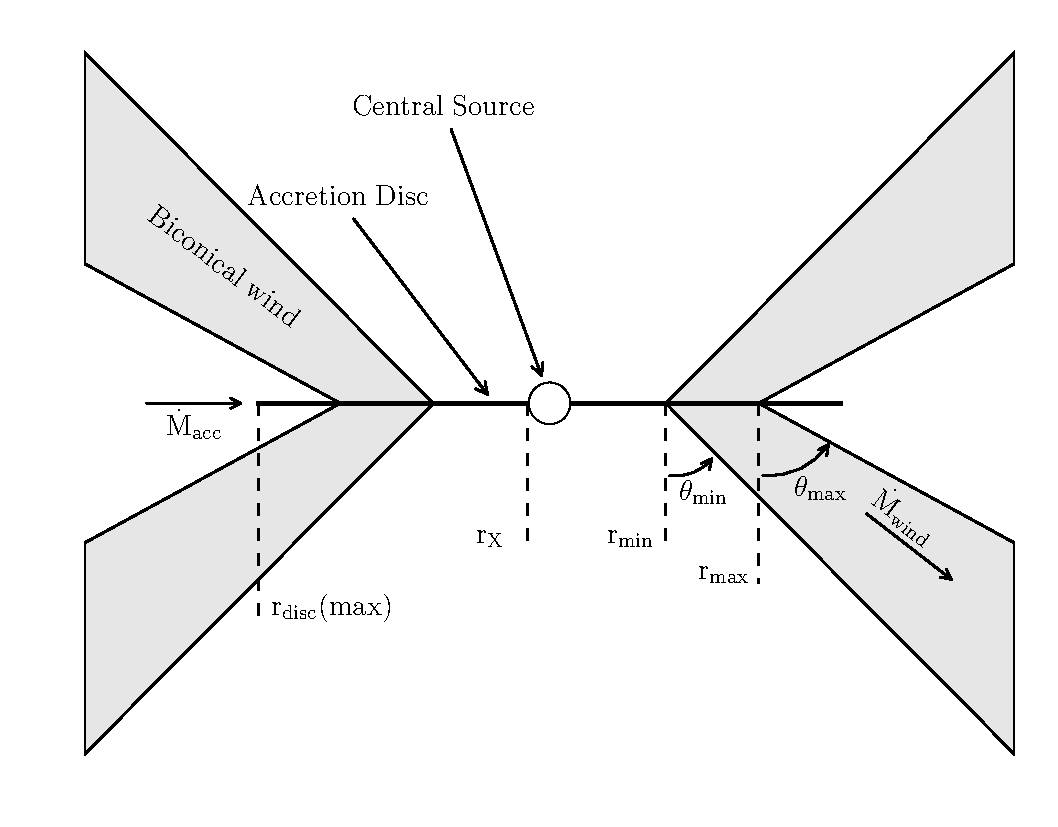
\includegraphics[width=0.45\textwidth]{figures/fig2_cartoon.eps}
\caption
{
A cartoon showing the geometry and some key parameters of
our biconical wind model.
}
\label{fig:cartoon}
\end{figure}



\subsection{A Benchmark Model for BALQSOs}

\cite{higginbottom2013} presented a benchmark model for
(BAL)QSOs...introduce key parameters. 

\subsubsection{Photon Sources}

Describe the photon sources in the model.

The accretion disc in our model is geometrically thin, but optically thick
and this adopt a standard multi-temperature blackbody
using a \cite{shakurasunyaev1973} temperature profile. 
The emergent SED is thus determined by the specified accretion rate ($\dot{m}$)
and central BH mass ($M_{BH}$).
The inner radius of the disc extends to the innermost stable circular orbit
(ISCO) of the BH. 
%% OUTER RADIUS? 
We assume a Schwarzchild BH with an ISCO at $6~R_G$.
The X-ray source in our model is treated as an isotropic sphere at the ISCO,
which emits photons according to a power law,

% \begin{equation}

% \end{equation}

% With a normalisation such that it produces the correct 2-10kev luminosity.

% Photons striking the 





% which successfully reproduced BAL features 
% in synthetic spectra using \py. However, the model
% had a few key drawbacks when considering its potential
% for unification. First, it failed to produce significant
% broad emission lines at non-BAL viewing angles; this is 
% a key requirement for a unified QSO model. Second,
% the model was significantly X-ray weak, as it was found
% that an X-ray luminosity comparable to that of a QSO 
% over-ionized the wind, resulting in no UV resonance 
% line absorption features.

% \begin{table}
% \begin{tabular}{p{3cm}p{4cm}}
% \hline Free Parameters 	&	 Value \\ 
% \hline \hline 
% $M_{BH}$ 	 &	 $1\times 10^9~\rm{M_{\odot}}$ \\ 
% $\dot{M}_{acc}$ 	 &	 $5~M_{\odot}yr^{-1} \simeq 0.2~\dot{M}_{Edd}$\\ 
% $\alpha_X$ 	 &	 $-0.9$ \\ 
% $L_{X} $ 	 &	 $1\times10^{43}~\rm{ergs~s^{-1}}$\\ 
% $r_{disc}(min)=r_{X}$   &	 $6r_g=8.8\times10^{14}~{\rm cm}$ \\ 
% $r_{disc}(max)$   &	 $3400r_g = 5\times10^{17}~{\rm cm}$ \\ 
% $\dot{M}_{wind}$  &	 $5~M_{\odot}yr^{-1}$ \\ 
% $r_{min}$ 	&	 $300r_{g} = 4.4\times10^{16}~{\rm cm}$\\ 
% $r_{max}$ 	&	 $600r_{g} = 8.8\times10^{16}~{\rm cm}$ \\ 
% $\theta_{min}$ 	&	 $70.0^{\circ}$ \\ 
% $\theta_{max}$ 	&	 $82.0^{\circ}$ \\ 
% $\lambda$ 	&	 $0$ \\ 
% $v_{\infty}$ 	&	 $v_{esc}$(f=1) \\ 
% $R_v$ 	        &	 $1\times10^{18}$cm \\ 
% $\alpha$ 	&	 $1.0$ \\
% \hline 
% Derived Parameters 	&	 Value \\ 
% \hline \hline
% $L_{\nu}(2500\mbox{\scriptsize{\AA}})$&	 $6.3\times10^{30}~\rm{ergs~s^{-1}~Hz^{-1}}$\\ 
% $L_{\nu}(2keV)$   &	 $1.2\times10^{25}~\rm{ergs~s^{-1}~Hz^{-1}}$\\ 
% $L_{bol}$ 	 &	 $2.4\times10^{46}~\rm{ergs~s^{-1}}$\\
% $M_{bol}$ 	 &	 -27.4\\ 
% $M_u$            &	 -26.2\\ 
%  $\alpha_{OX} $ 	 &	 -2.2\\ 
% \end{tabular}
% \caption{Wind geometry parameters used in the benchmark model.}
% \label{wind_param}
% \end{table}

\subsection{Potential for unification}

What was wrong with H13 model - X-rays + BELs.

\subsection{Clumping}

Introduce microclumping.

% To take account of clumping in our outflow we adopt a simple parameterization
% used in stellar wind modelling, known as {\em microclumping} \citep{hamann1998}. 
% The key assumption here is that typical clump sizes
% are much smaller than the typical photon mean free path, and thus the clumps are 
% both geometrically and optically thin. This approach is typically 
% known as microclumping and allows one to introduce a `filling factor', $f$, which is the 
% fraction of the volume of the plasma filled by clumps. We can then introduce the 
% density enhancement, $D$, which is simply 

% \begin{equation}
% D = \frac{1}{f}
% \end{equation}

% One can then multiply all densities in the model by $D$, and all emitting volumes
% by $f$, meaning that all $\rho^2$ processes 
% (such as collisional excitation and recombination) will be enhanced, 
% while opacities remain unchanged (for fixed ionization state). A factor $f$ is also
% applied to the opacities such that opacities which scale only with $\rho$ are not
% increased. Clumping the wind has an important effect on the ionization state and has
% been proposed as a solution to the so-called `over-ionization problem' in 
% disc winds (refs). This is the main motivation for incorporating microclumping
% into our model.  



%%%%%%%%%%%%%%%%%%%%%%%%%%%%%%%%%%%%%%%%%%%%%%%%%

% RESULTS

%%%%%%%%%%%%%%%%%%%%%%%%%%%%%%%%%%%%%%%%%%%%%%%%%

\clearpage

\section{Results}


\begin{figure*}
\centering
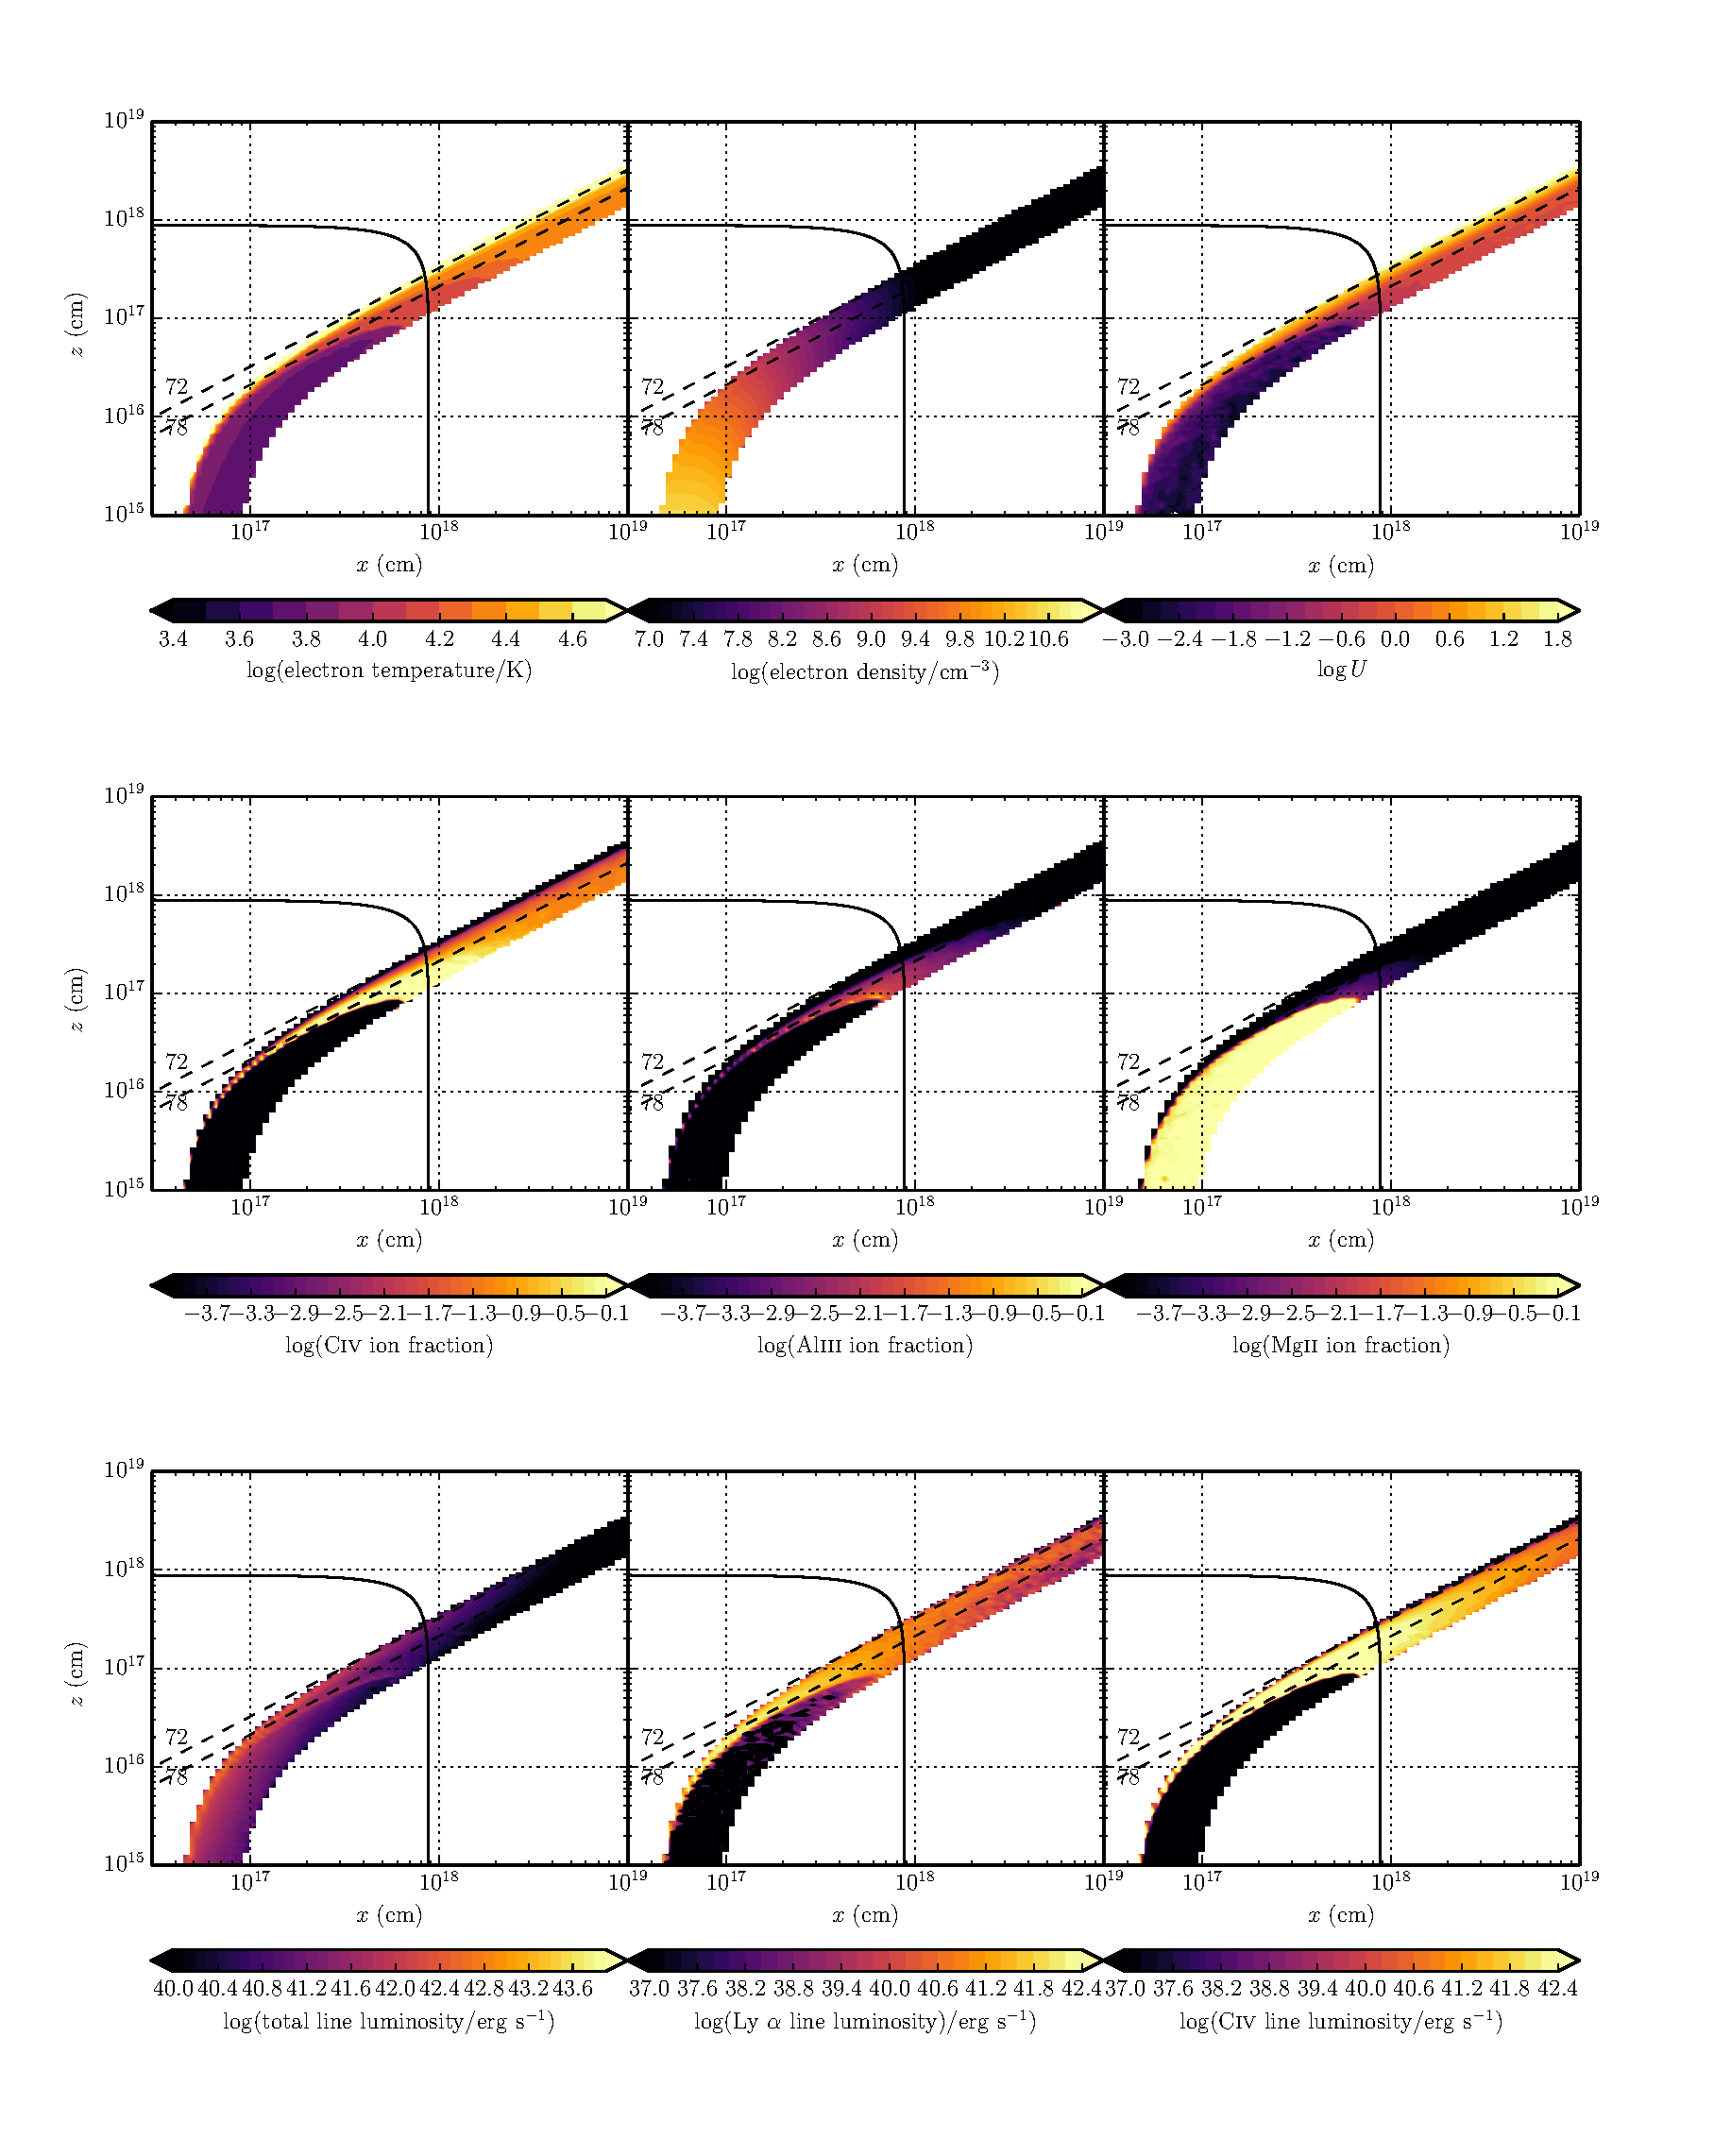
\includegraphics[width=1.0\textwidth]{figures/wind.eps}
\caption
{
Physical properties of the outflow.
}
\label{fig:uvspec}
\end{figure*}

\begin{figure*}
\centering
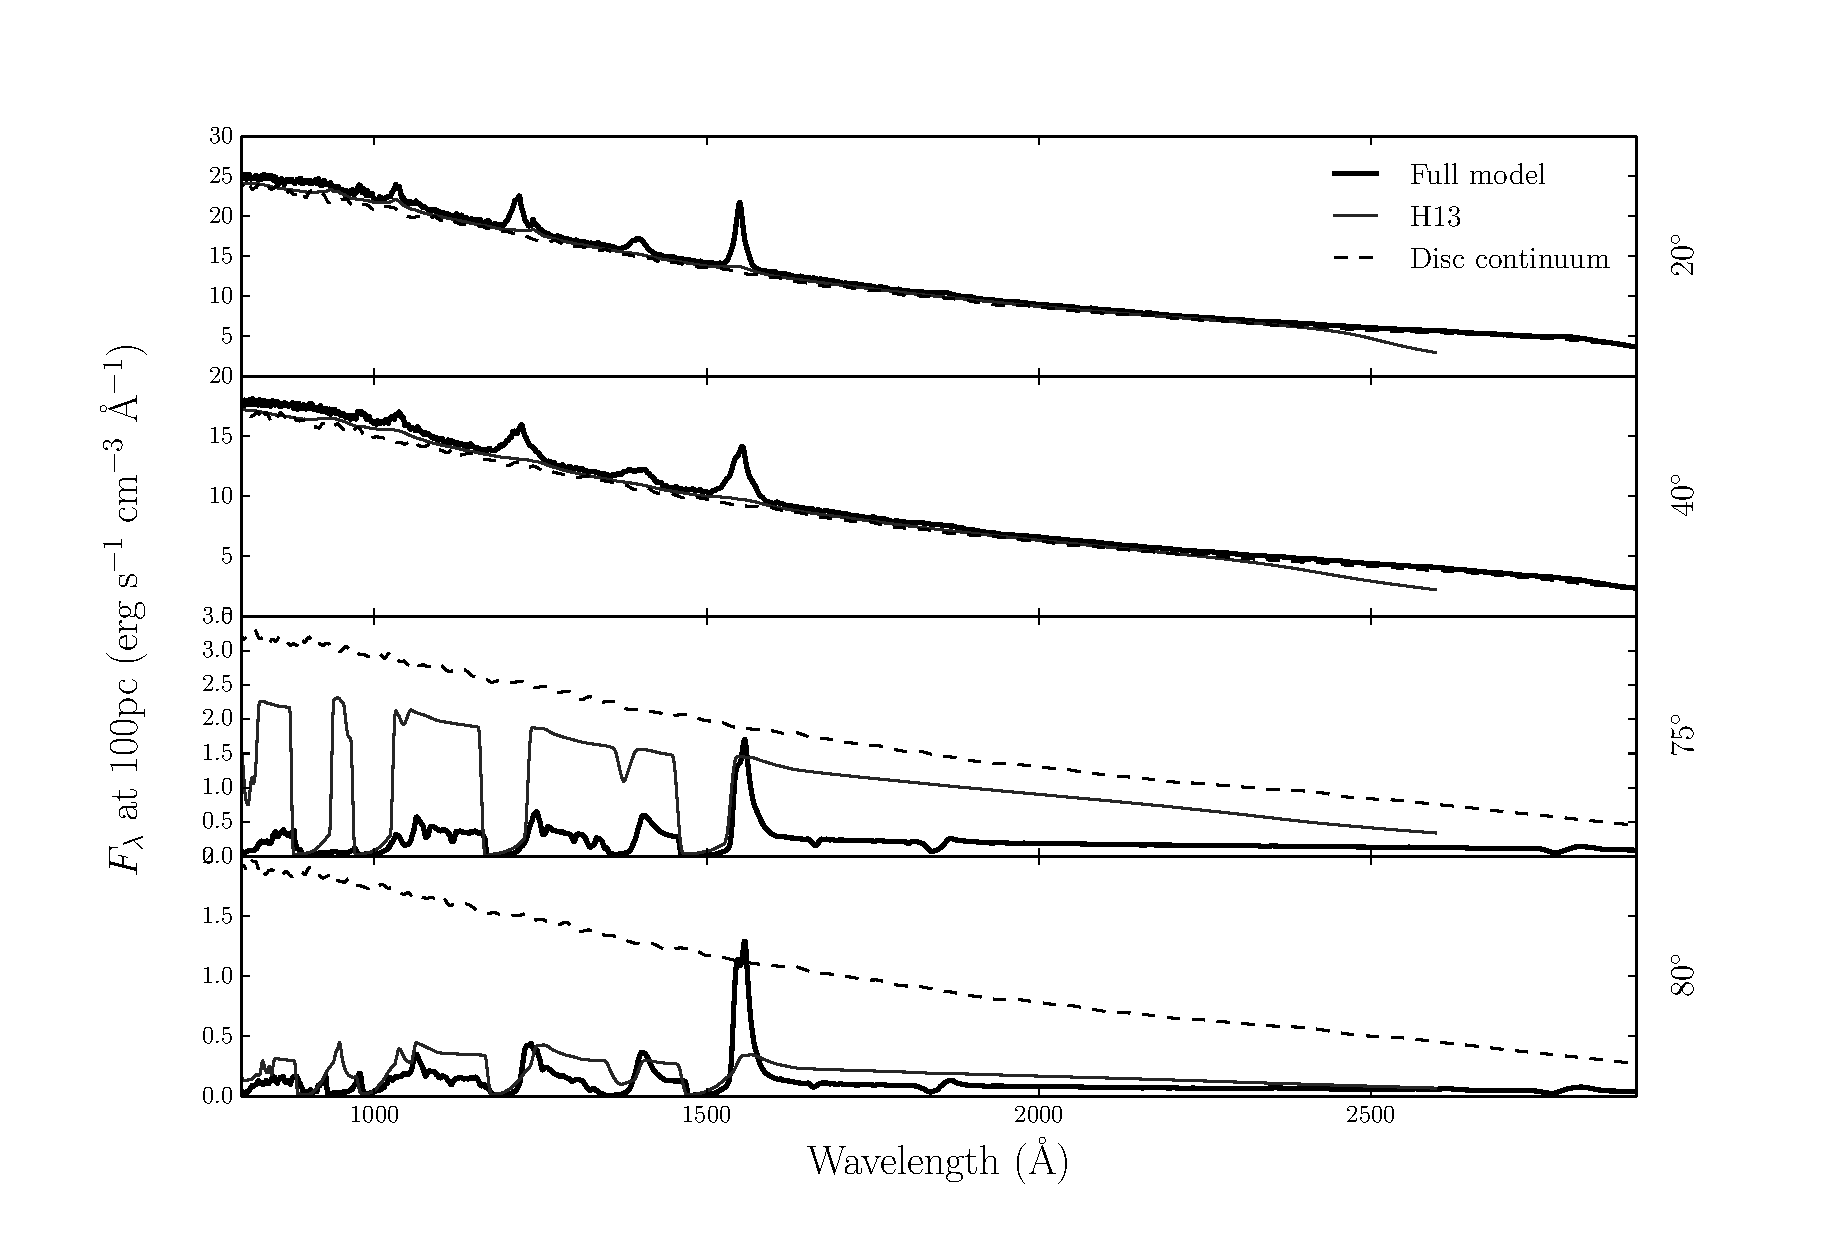
\includegraphics[width=1.0\textwidth]{figures/uvspec.eps}
\caption
{
Synthetic spectra at four viewing angles in the clumpy model. Plot would look different probably,
and may show composites, but this would be the main synthetic spectrum plot.
}
\label{fig:uvspec}
\end{figure*}

\begin{figure*}
\centering
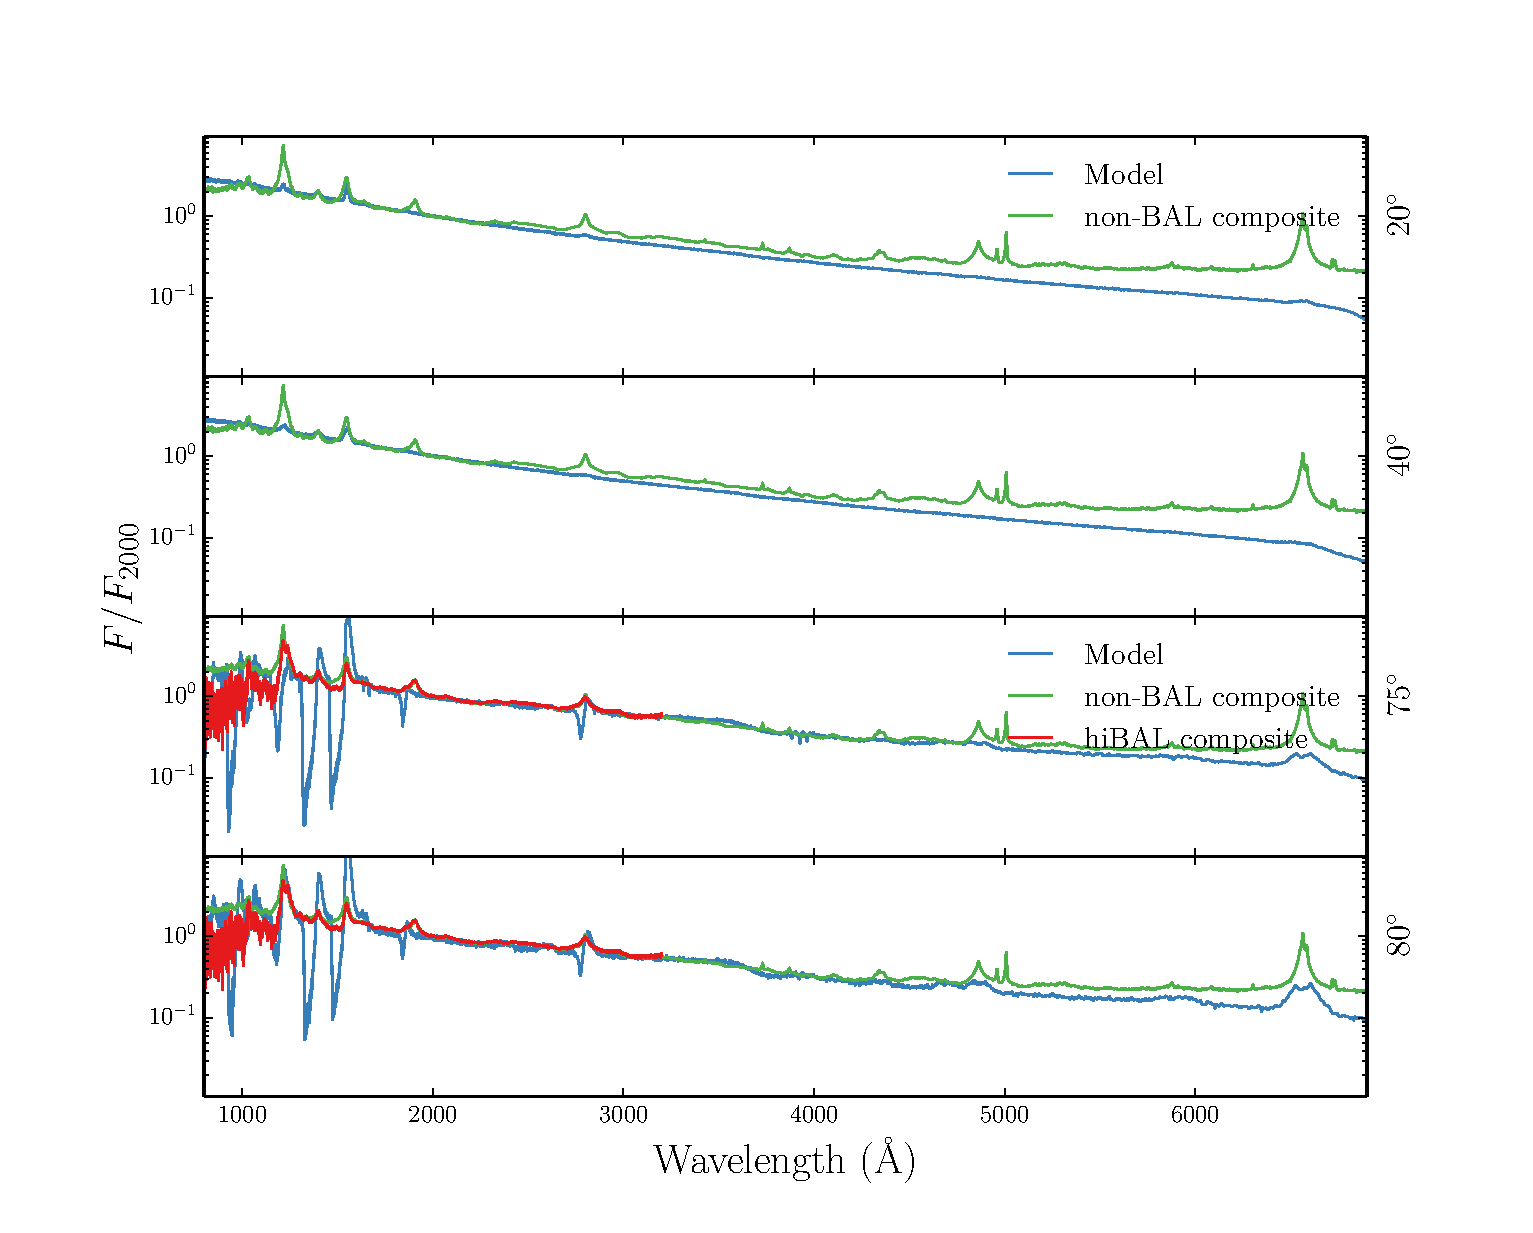
\includegraphics[width=1.0\textwidth]{figures/opt.eps}
\caption
{
Figure designed to show optical spectrum and comparison to composite.
}
\label{fig:uvspec}
\end{figure*}

\begin{figure*}
\centering
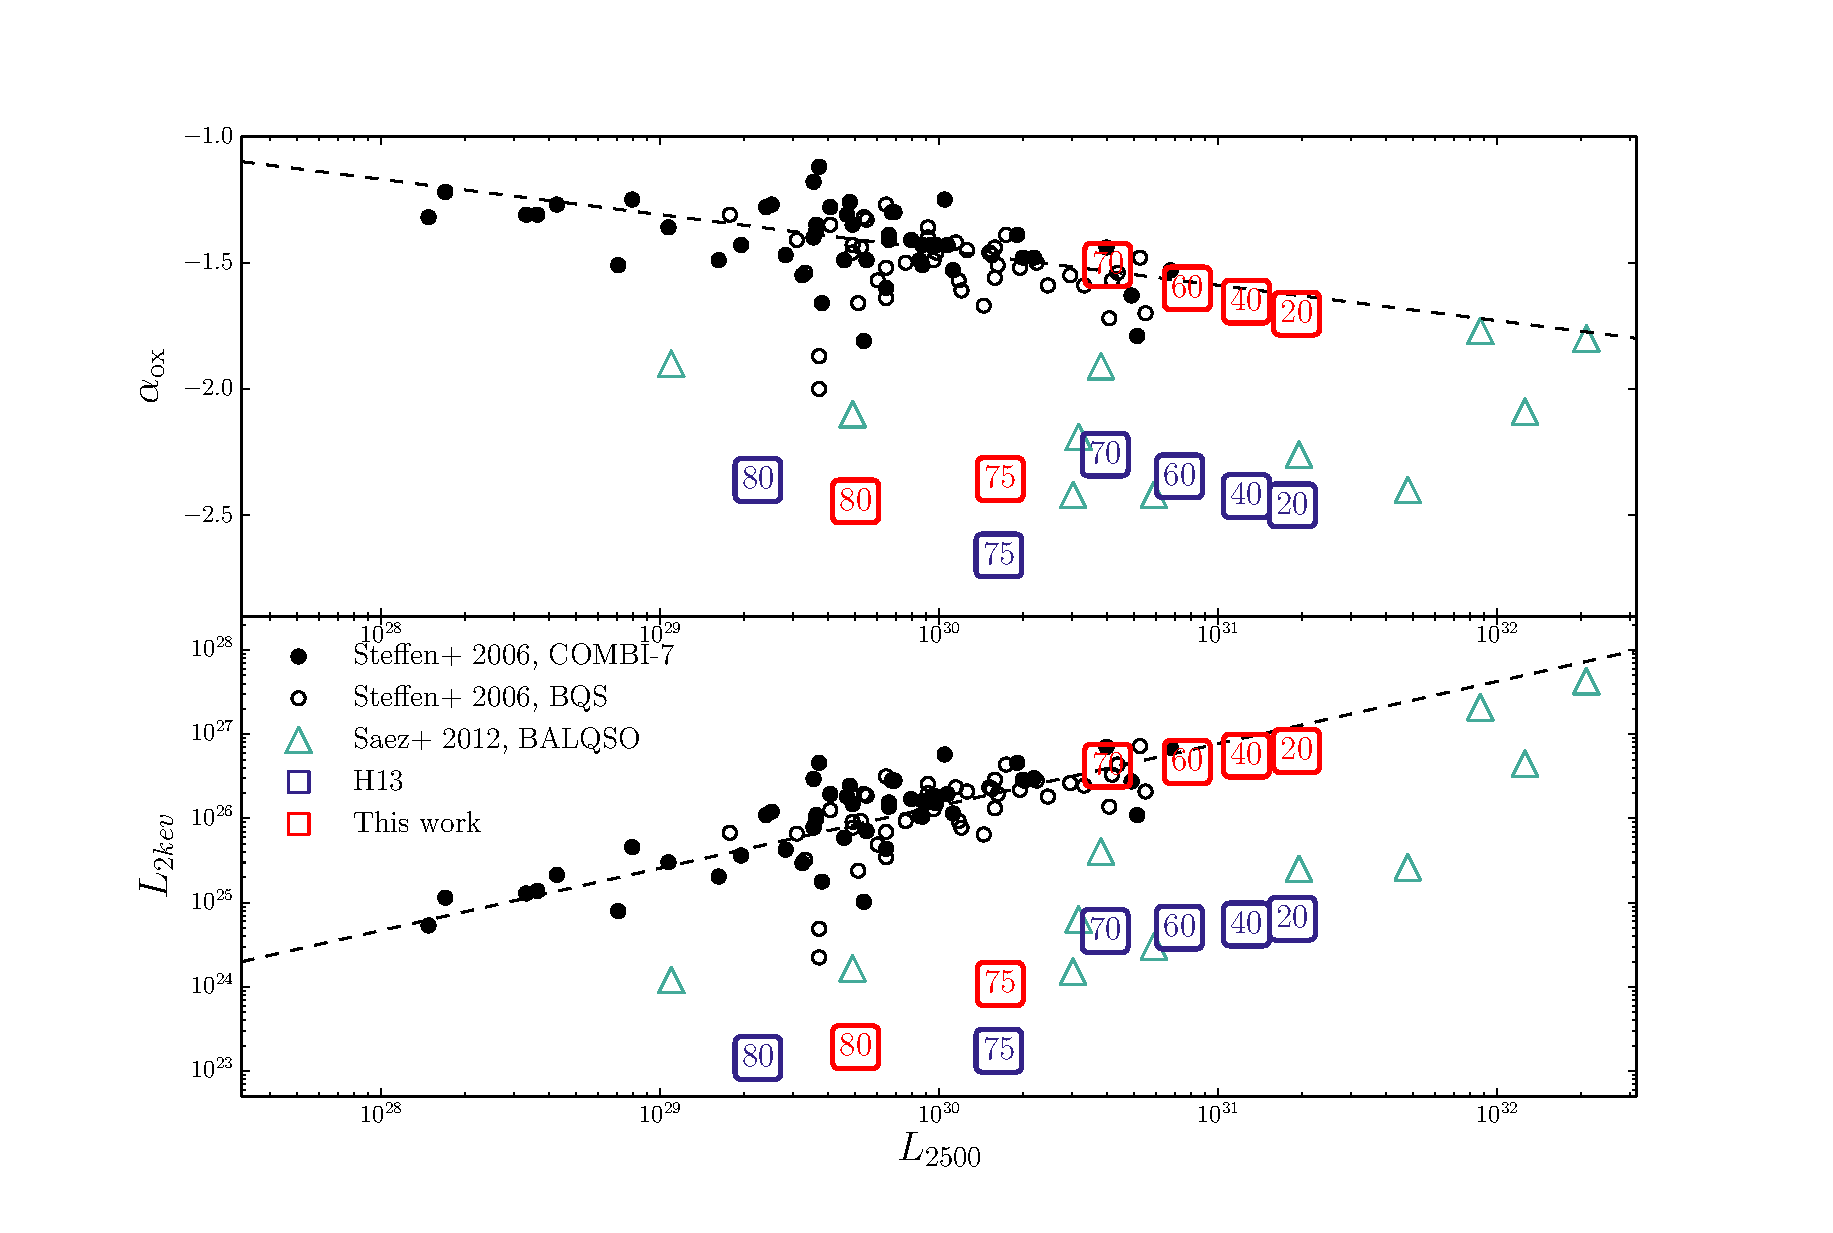
\includegraphics[width=1.0\textwidth]{figures/alpha_ox_both.eps}
\caption
{
X-ray properties of the H13 and clumped model (text filled 
squares), plotted against monochromatic luminosity 
at 2500\AA. Also plotted are the samples considered by
Saez et al. 2012 on a similar plot; The COMBI-7 AGN sample (ref),
the BQS sample (ref) and the Saez et al. (2012) sample of BALQSOs.
}
\label{fig:xray}
\end{figure*}

\subsection{Physical Conditions and Ionization State}

Show that clumping stops over-ionization.


{\bf Figure 2: Physical conditions of the wind, showing e.g. CIV fraction.} 

\subsection{Synthetic Spectra}

Present a spectrum of the UV and possible optical too. 


{\bf Figures 3 and 4: UV and optical spectra.} 

\subsection{X-ray Properties}

discuss the figure showing X-ray properties briefly. 
Present an X-ray spectrum? compare to observations e.g. Giustini?

{\bf Figures 5 and 6: $L_{2kev}$ v $L_{2500}$ plot and X-ray spectrum compared to Grupe and Nousek (broadband SED?)} 

\subsection{LoBALs and trends with inclination}

{\bf Figure 7: line profiles of CIV, Mg II and Al III as a function of inclination.} 


\begin{figure}
\centering
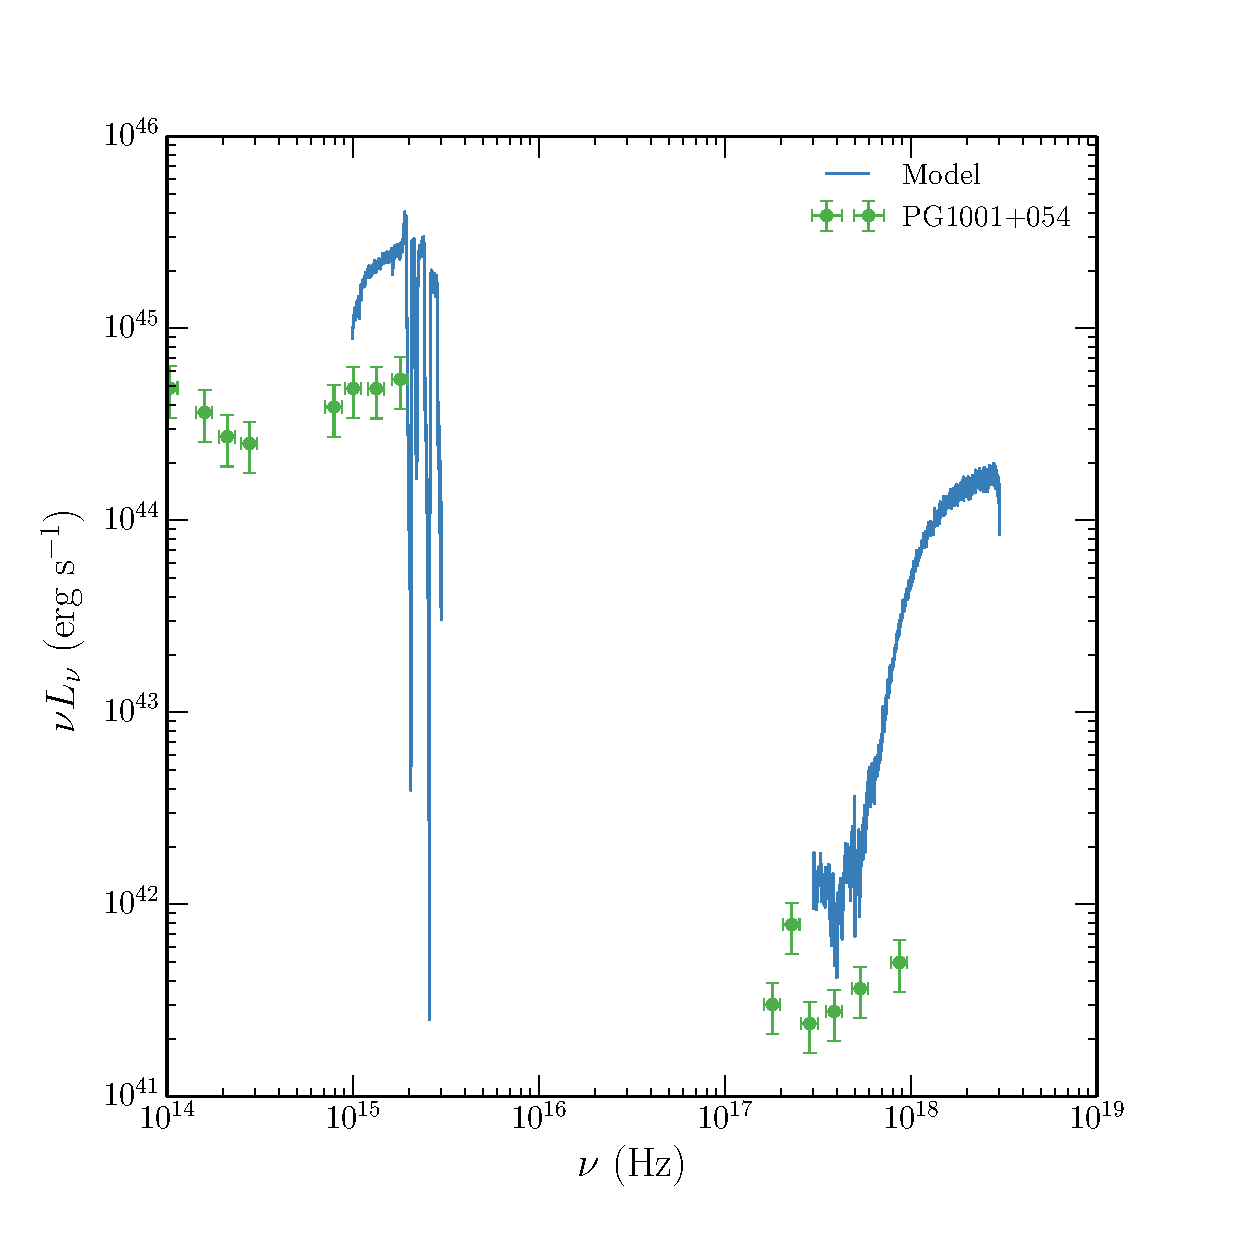
\includegraphics[width=0.5\textwidth]{figures/xray_spectrum_lnu.eps}
\caption
{
Broadband SEDs compared to IR and X-ray SEDs for selected BALQSOs 
from Grupe \& Nousek (2015).
}
\label{fig:xray}
\end{figure}


\begin{figure*}
\centering
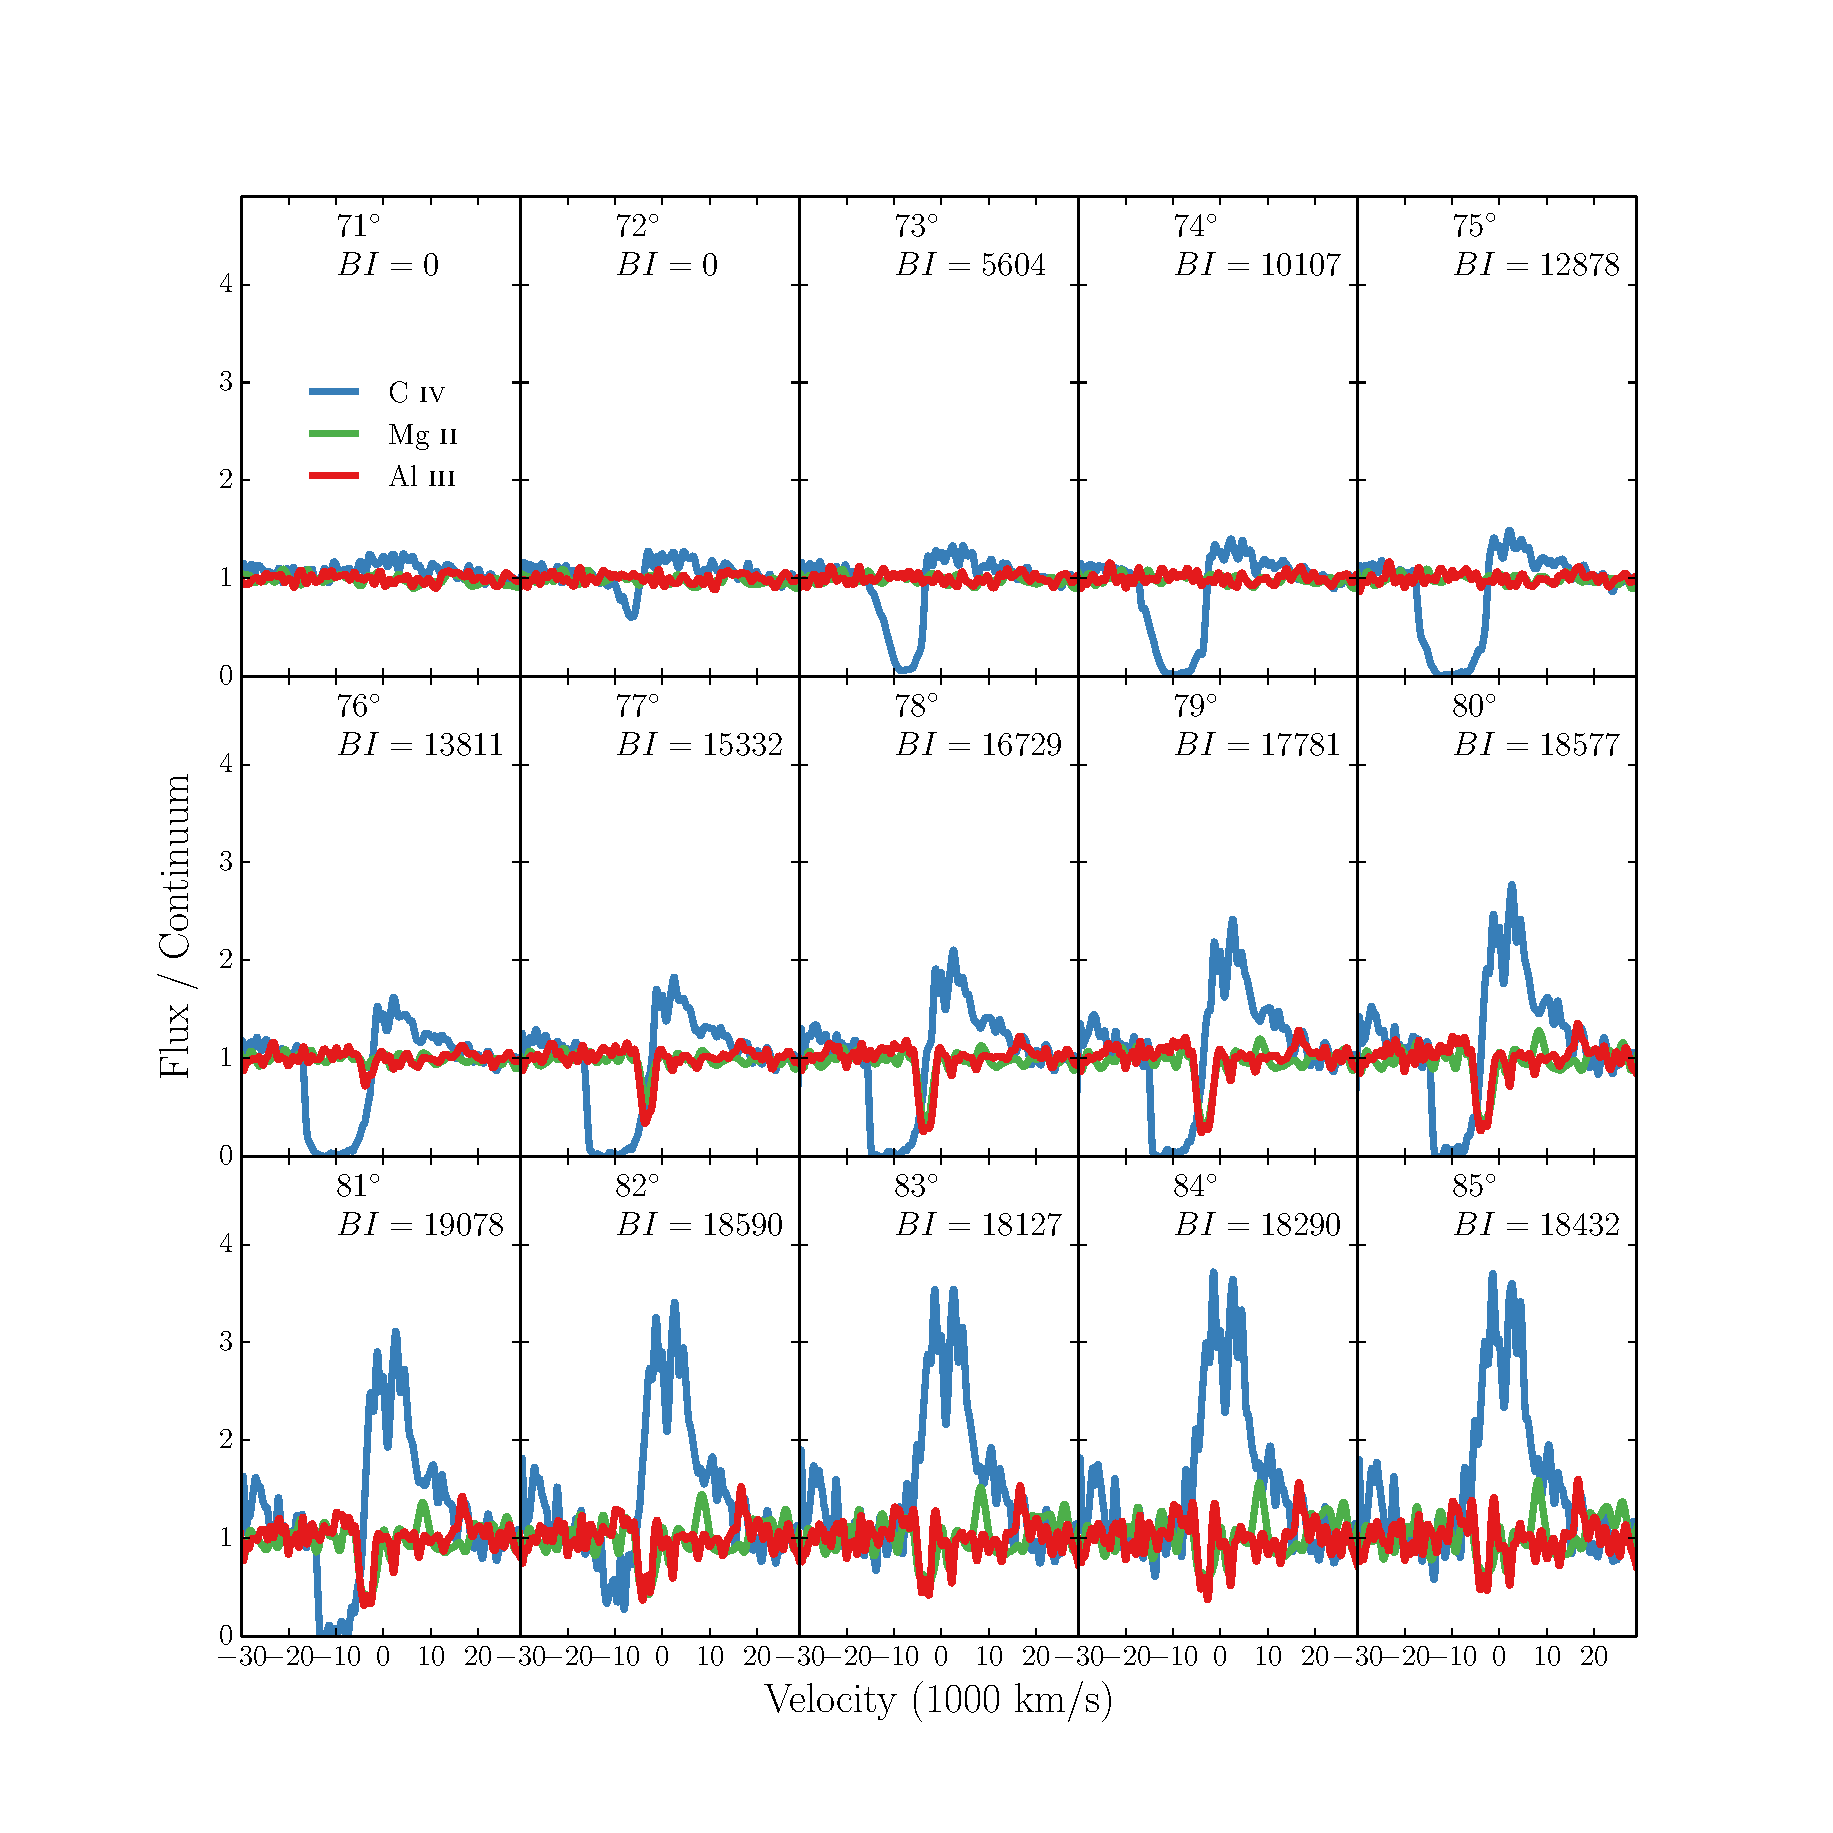
\includegraphics[width=1.0\textwidth]{figures/c4_with_i.eps}
\caption
{
Carbon IV, Al III and Mg II line profiles with inclination for wind angles.
Showing how the line profiles change
and how LoBALs kick in at particularly high inclinations.
}
\label{fig:xray}
\end{figure*}


%%%%%%%%%%%%%%%%%%%%%%%%%%%%%%%%%%%%%%%%%%%%%%%%%

% DISCUSSION 

%%%%%%%%%%%%%%%%%%%%%%%%%%%%%%%%%%%%%%%%%%%%%%%%%

\clearpage
\section{Discussion}

\subsection{Anisotropy of disc emission}

Discuss the importance of the angular distribution of the disc SED on line
(limb-darkened, foreshortened, etc.)

\subsection{General relativistic effects}

Can GR effects offer a potential solution? (not quite!)

{\bf Figures 8 and 9: AGNSPEC F(2000) as a function of viewing angle compared to a BB disc.
spectrum compared to composites with AGNSPEC correction.} 

\begin{figure}
\centering
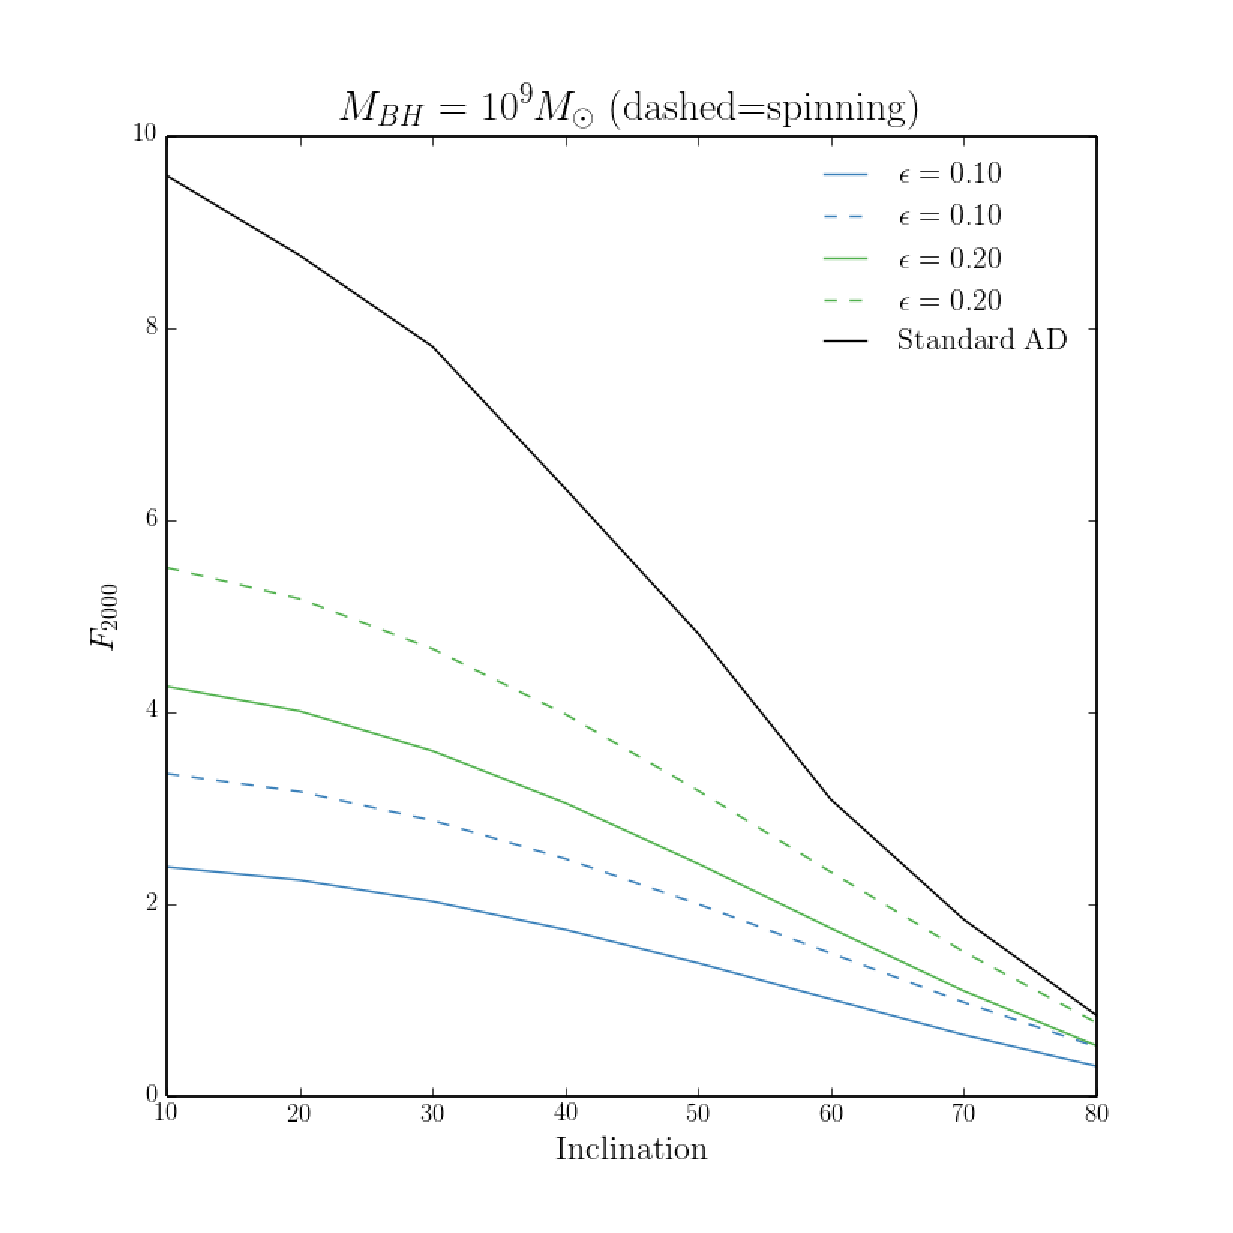
\includegraphics[width=0.5\textwidth]{figures/f2000_m9.eps}
\caption
{
$F_{2000}$\ as a function of inclination from
\agn\ models, compared to a classical AD. 
{\bf This is a placeholder- it will show the effect of GR on the anisotropy
of the disk for different wavelengths and eddington fractions, compared
to limb darkened and foreshortened classical AD}.
}
\label{fig:f2000}
\end{figure}


\begin{figure*}
\centering
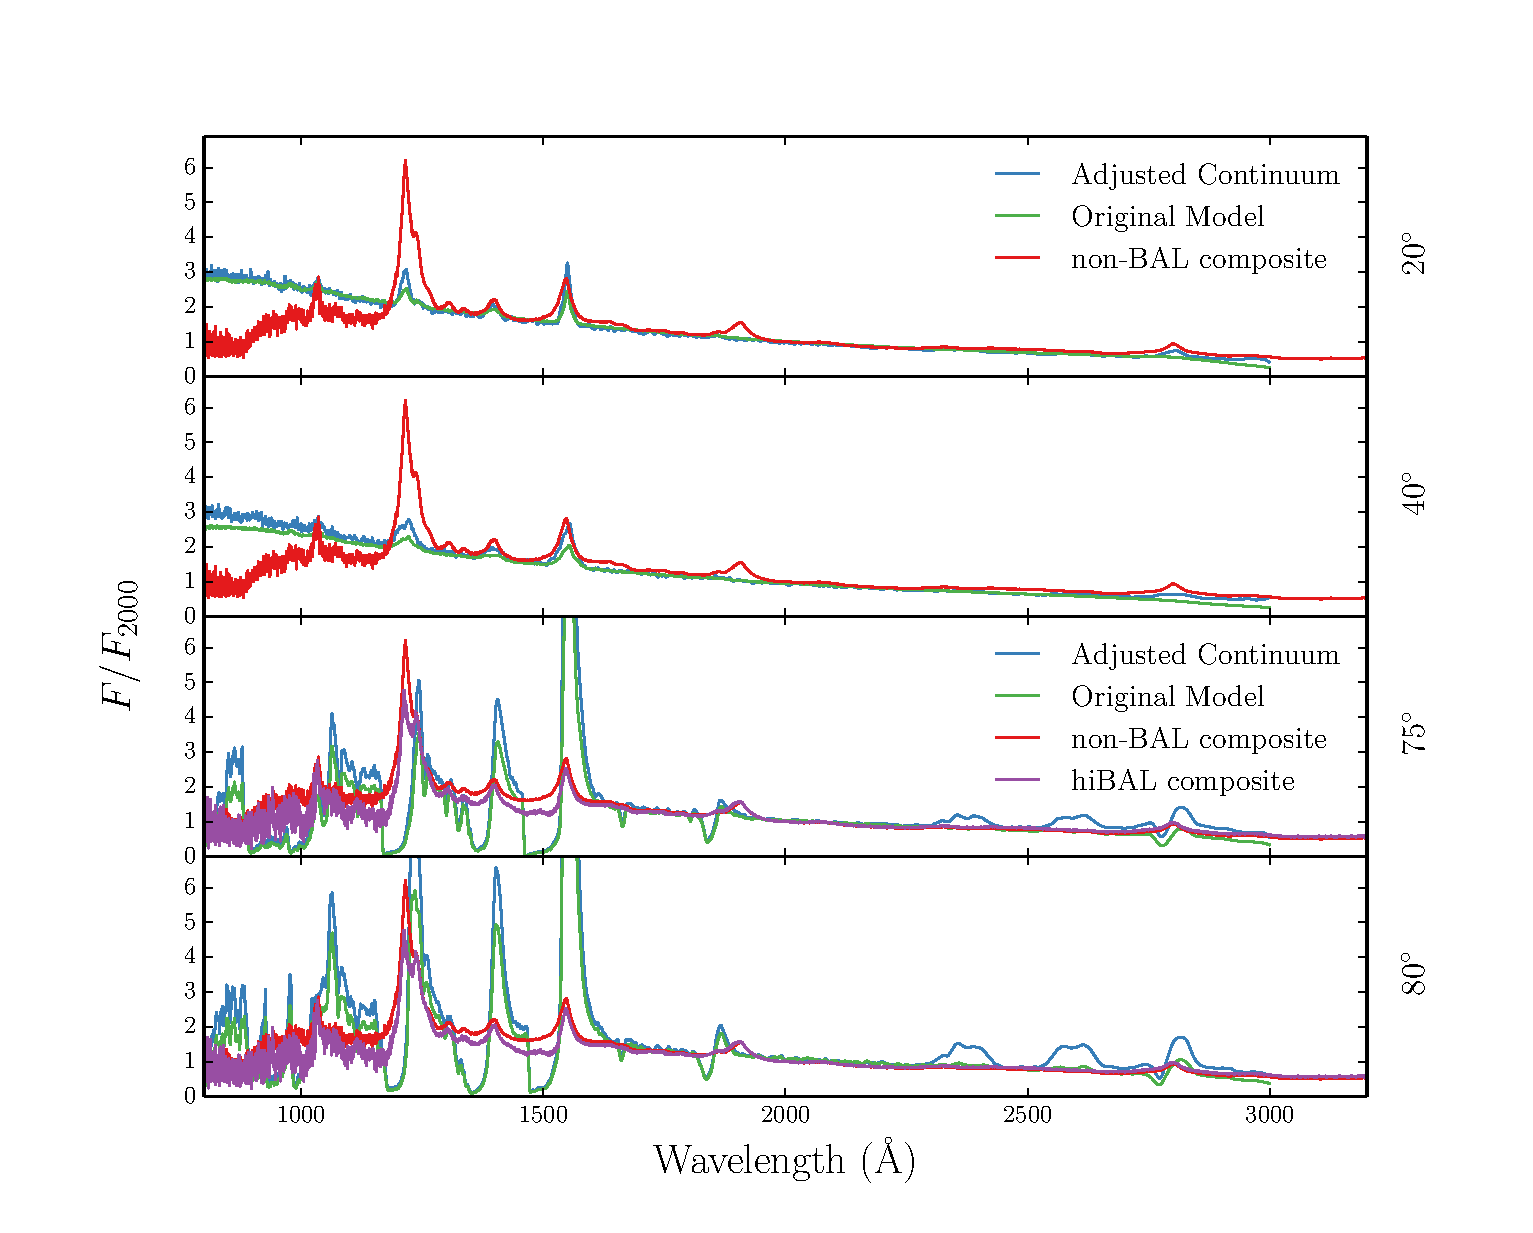
\includegraphics[width=1.0\textwidth]{figures/adjusted_withbals.eps}
\caption
{
$F_\lambda$ normalised to $F_{2000}$. {\bf Again, this is a placeholder- but I'm thinking some kind of comparison to composite including the adjusted continuum, showing that we can't get it exactly right}.
}
\label{fig:finalcomp}
\end{figure*}

\subsection{Wind reprocessing}

How would wind reprocessing help?

\subsection{The BALQSO fraction and wind covering factor}

A brief comment, citing Goodrich / Krolik \& Voit on the 
way in which anisotropy / attenuation affect the inferred
BAL fraction. We also need to be aware that there will be a number of selection
effects in building up the composites, and we should discuss these
and the subtleties involved. 

% \begin{figure}
% \centering
% 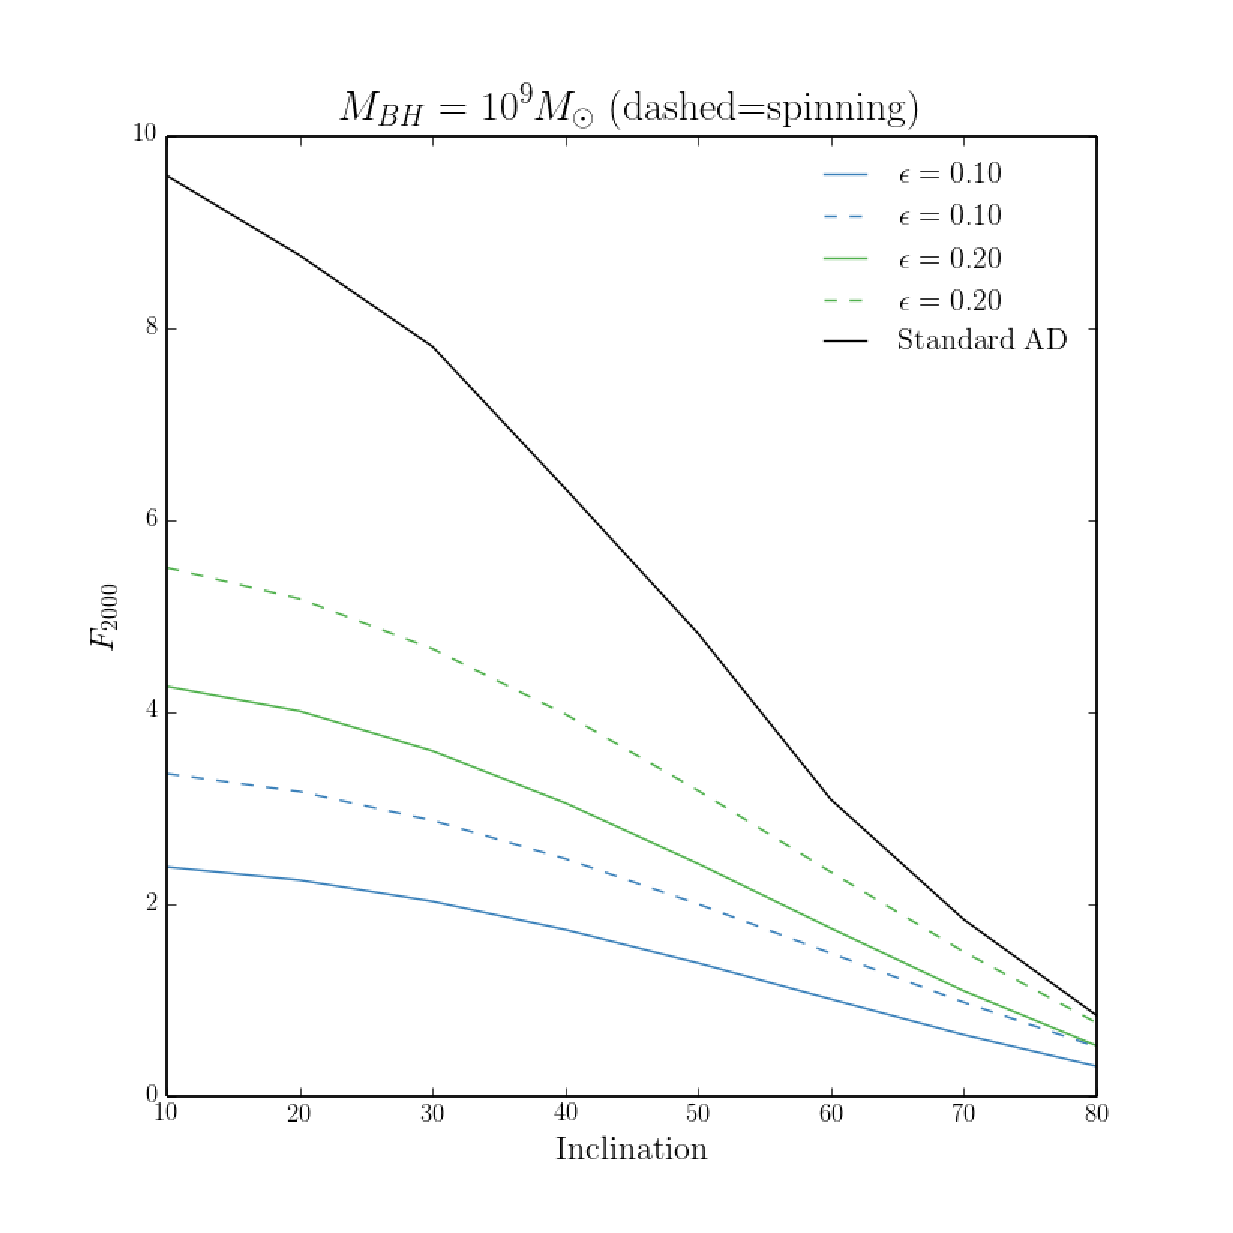
\includegraphics[width=0.45\textwidth]{figures/f2000_m9.eps}
% \caption
% {
% $F_\lambda$ at $2000$~\AA\ as a function of inclination from
% \agn\ models. Spectra are computed for BH of $10^9~M_\odot$ with
% a number of different BH spins and Eddington fractions. The black line
% shows a standard multi-temperature blackbody AD model.
% }
% \label{fig:alpha_ox}
% \end{figure}


%%%%%%%%%%%%%%%%%%%%%%%%%%%%%%%%%%%%%%%%%%%%%%%%%

% SUMMARY

%%%%%%%%%%%%%%%%%%%%%%%%%%%%%%%%%%%%%%%%%%%%%%%%%
\newpage
\section{Summary}

We have carried out MCRT simulations using a simple
prescription for a biconical disc wind, with
the aim of expanding on the work of H13 and assessing 
the viability of such a model for geometric unification of quasars.
We find the following main points:

\begin{enumerate}
\item We have introduced a simple, first-order treatment 
of clumping in our model, and found that it can now maintain
the required ionization state while agreeing well with the X-ray
properties of AGN/QSOs.
\smallskip
\item We find that clumping also causes a significant 
increase in the strength of the  emission
lines produced by the model. This is true both
of collisionally excited resonance lines (such as \civ, \nv)
and recombination lines (such as \la, \ha\ and the Balmer series).
\smallskip
\item The line EWs in our models are not comparable to those in Quasar composite
spectra. This is due to a fundamental constraint discussed in section ?. If the BLR
emits fairly isotropically then for a foreshortened, limb-darkened classical thin accretion disc
it is not possible to achieve line ratios at low inclinations that are comparable to
those at high inclinations. This is a robust conclusion which 
is independent of the assumed BLR geometry. 
\smallskip
\item We have examined the effect of GR on our disc SED, using the disc atmosphere
and GR ray-tracing code \agn. While including GR effects
does cause the disc SED to become significantly more isotropic,
the effect is not large enough to produce uniform line to continuum ratios
with viewing angle. We discuss other solutions to this problem in section ?; 
It is possible that a combination of GR and reprocessing by the wind could provide a 
solution, and a number of complicated selection effects may be at work
in the building of the quasar composites.
\end{enumerate}

Our work confirms a number of expected outcomes from such a model, and suggests 
that a simple geometry such as this can come close to explaining much of the 
phenomenology of quasars. Nevertheless, our conclusions pose a clear challenge 
to the current unification picture.


\section*{Acknowledgements}

%% \texttt{mn2e.cls} \textsc{Latex} document class. 


\bibliography{mybib.bib,stellar.bib,h14.bib,h13.bib}
\newpage
%\appendix
\end{document}
